% !TEX root = Final_Report.tex

\section{Finite Magnetic Field}
\label{sec:finite_field}

Having explored the finite-temperature predictions for the soft-constraint in the absence of a magnetic field, we now introduce a finite magnetic field $ B $ which breaks the previous isotropy of the problem. One can include the effects of the magnetic field by introducing a Zeeman term for the magnetic impurity \cite{LargeN}: $$ F_{B} = - g \mu_{B} B \left( f^{\dagger}_{\uparrow} f^{}_{\uparrow} - f^{\dagger}_{\downarrow} f^{}_{\downarrow} \right) \cong - g \mu_{B} B \sum_{\sigma} \sigma p^2_{\sigma} ~ , $$ where $ g $ is the \textit{g-factor} and the effect on the conduction electrons is irrelevant at this scale.

\subsection{Effect on the Mean-Field Equations}

The inclusion of a magnetic field leaves the previous mean-field equations of Section~\ref{subsec:obtaining_MF} largely unchanged apart from the equation for the singly-occupied KR boson, which now becomes
\begin{equation}
\frac{\partial F}{\partial p_{\sigma}} = 0 \implies \sum_{s} \left[ \frac{\partial F_{0}}{\partial \xi_{s}} - \frac{\partial F_{0}}{\partial \overline{\xi_{s}}} \right] \frac{\partial z^2_{s}}{\partial p_{\sigma}} ~ i \Delta = - p_{\sigma} ~ (\lambda_{\text{KR}} - \lambda_{\sigma} - \sigma g \mu_{B} B) ~ .
\end{equation}
Without isotropy, however, solving the mean-field equations becomes appreciably more difficult, and so we will restrict ourselves to the slightly simpler task of searching for the location of the phase boundary $ \Delta = 0 $ in the $ B-T $ plane because it allows particle-hole symmetry to be justifiably used again.
% Maybe add an appendix in which you show that particle-hole symmetry works at \Delta = 0

\subsection{Plotting the Phase Boundary}

Setting $ \Delta = 0 $, the mean-field Lagrange multipliers are found to be:
\begin{equation}
\lambda_{\text{KR}} = 0 ~, \quad \lambda_{\text{SC}} = 0 ~,
\quad \lambda_{\sigma} = - \sigma g \mu_{B} B ~.
\end{equation}
Proceeding with this fixed $ B $-field, we obtain the condition that the occupancy of the impurity is given by
\begin{equation}
p^2_{\sigma} = \frac{1}{2} ( 1 - \kappa ) + \sigma \frac{1}{\pi} \Im{\left[ \psi\left( \frac{1}{2} + \frac{g \mu_B B}{2 \pi i T} \right) \right]} ~,
\end{equation}
which in the large $ B $ limit will have $ \Im{\left[ \psi\left( \frac{1}{2} + \frac{g \mu_B B}{2 \pi i T} \right) \right]} \rightarrow - \frac{\pi}{2} $ such that $ p^2_{\downarrow} $ becomes negative. Physically, this corresponds to one spin-state of the impurity being heavily favoured compared to the other, but this mean-field solution requires intervention with a piecewise definition to ensure that both $ p^2_{\sigma} $ saturate sensibly.
% Stop using the word problematic so much

Making a parametric plot of the phase boundary in terms of $ b = \frac{g \mu_B B}{T} $ according to
\begin{equation}
\left( \frac{T}{T_K} \right) = \frac{1}{2 \pi \sqrt{\rho J}} e^{\left( 1 - z^{-2} \right) / (\rho J)} \exp{\left[ - \Re ~ \psi \left( \frac{1}{2} + \frac{b}{2 \pi i} \right) \right]} \quad \text{and} \quad \frac{g \mu_B B}{T_K} = \left( \frac{T}{T_K} \right) b
\label{eq:phase_parametric}
\end{equation}
reveals a more worrisome problem with this approach, namely that the behaviour is dominated by the $ \frac{1}{\rho J z^2} $ that appears in the exponential. If $ \kappa $ is left constant, then this leads to a phase boundary that curves upwards at large magnetic fields, as shown in Figure~\ref{fig:new_phase_boundary}, because $ z^2 $ includes other field-dependent terms.\footnote{This strange phase boundary does not arise if one is actually interested in the case where $ B $ is not fixed, but rather a uniformly distributed stochastic field $ \widetilde{B} \in [ - B / 2, ~ B / 2 ] $, since the imaginary part of $ \widetilde{\psi} (g \mu_B \widetilde{B}) $ averages to zero and the same large-N limit of the phase boundary is recovered for constant $ \kappa $.} This is despite the fact that the rest of the expression behaves similarly to the large-N limit found by Piers Coleman \cite{ManyBodyPhysics}, which was used to create the original phase diagram of Figure~\ref{fig:phase_diagram}.

\begin{figure}
\centering
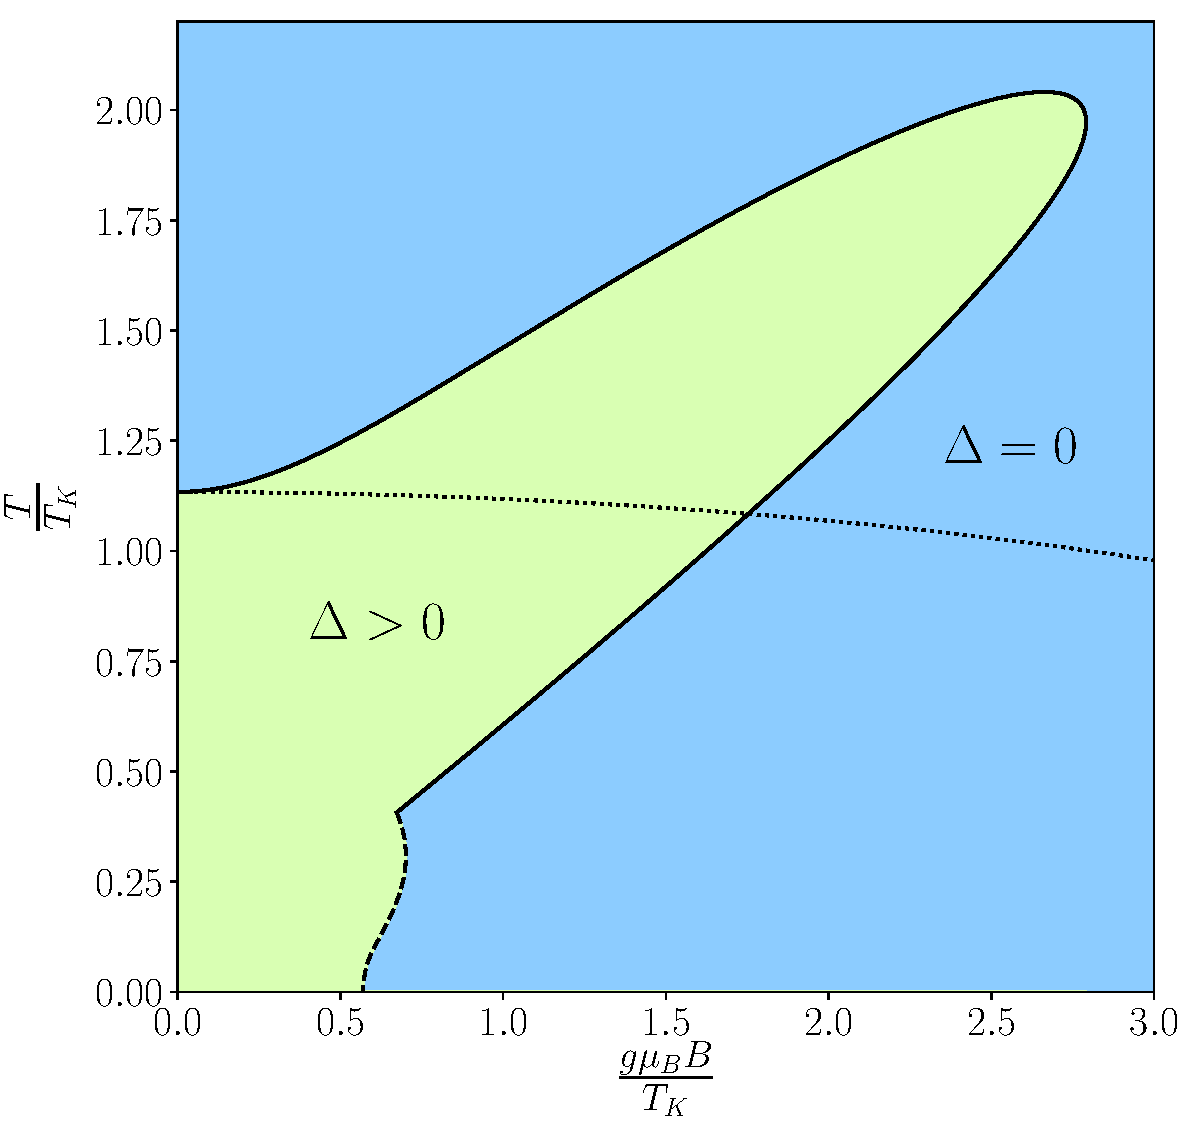
\includegraphics[width=0.7\textwidth]{Figures/new_phase_diagram.pdf}
\caption{A phase diagram for the soft-constraint approach when $ \kappa $ held constant, generated parametrically using Eq~\eqref{eq:phase_parametric}. The shape of the boundary is highly sensitive to $ z^2(\frac{B}{T}) $, which is itself made to saturate by-hand beyond a certain value of $ \frac{B}{T}$ and is plotted as a dashed line thereafter to indicate that it is no longer the true mean-field boundary. The dotted line shows the original large-$N$ boundary of Figure~\ref{fig:phase_diagram}.}
\label{fig:new_phase_boundary}
\end{figure}
% Need to have the form of z^2 in the appendix

If one is truly interested in the case of the Kondo model subject to a fixed magnetic field, then it appears that $ \kappa $ would have to acquire a (likely complicated) $B$-field dependence to tame this unexpected behaviour. Given that it was only ever possible to increase the order of the phase transition in the absence of a magnetic field, it seems likely that a phase transition is also inevitable at finite fields. (Even the task of increasing the order of a phase transition is made much more challenging at finite field, and so has not been attempted in this project.)

% Go through your result for the phase-boundary when K is constant, then frame it as if constant K is once again usatisfactory

% Mention that you could have done something similar where you average over the stochastic field, which makes z^2 into a constant thing so that you get back to the large-N limit

% Say that you haven't worked out how you would go about changing k at finite field to get a sensible curve

% Maybe add an appendix in which you show that particle-hole symmetry works at \Delta = 0

% Mention the way that a magnetic field can be included in an ad-hoc way
% Show that it is problematic unless you define a stochastic field
% Or just make the p_\sigma s saturate at zero? - Doesn't work